\documentclass[11pt]{article}

% This package sets the margins to 1in
\usepackage{fullpage}
\usepackage{graphicx}
\usepackage{multicol}

\title{Project 2}
\author{Bill Collins and Alec Gerhart}
\date{April 29, 2016}
\begin{document}
\begin{multicols}{2}

\maketitle


\center 
Abstract
\flushleft



\center 
Problem Description 
\flushleft

Predicting the growth and depletion of a population has been important in keeping societies alive. In most governments today, populations are regularly checked to update the state of a nation. The goal of our next-event simulation is to create a virtual population on a 50x50 grid that can feed and reproduce so that we can find patterns in how a society can sustain itself. This will allow us to see limits in population growth and decay, and may allow us to find an average amount of members in the population of this very basic society.


\center 
Validation and Verificaiton
\flushleft
To create our simulation, we first had to create the members of our population. We will refer to these members as agents.

Agents search within their field of view for the location on the grid that has the most food. They travel to this location to pick up the food. If the agent is fertile, it will also look for an agent of the opposite gender to reproduce with. If the agent runs out of food, then it starves to death. If the agent never starves to death, then it will die of old age. \newline

We created an agent class that would represent an agent. The agent's constructor took in the current time (the time that the agent was created), the agent's unique id, and its location on the grid (x and y coordinates). These values were all saved in the agent object, and other values were created within the constructor. The agent has a variable that tells whether or not it is alive, which starts at True. When the agent dies, we set this value to false. The agent's gender is determined by Bernoulli(0.5), where they are male if this value is 1. The agent becomes fertile at a time determined by Uniform(12, 15). If the agent is male, then their fertility ends at Uniform(40, 50). If the agent is female, then fertility ends at Uniform(50, 60). The agent's metabolism, which is how quickly their food decreases, is determined by Uniform(1, 4). The agent loses this amount of food for each unit of time that passes. As stated before, the agent can die of old age. This age is determined by Uniform(60, 100). The agent also has a pregnancy variable, which is true if the agent or its mate is pregnant, and is false otherwise. The agent also has a field of view, which is an Equilikely value between 1 and 6, and represents how far an agent can see.
The agent also starts with wealth, or food-level, of 100.
\newline
Later on, we decided to add evolution to the agents of the simulation. If the agent has parents (it is not part of the first generation), then its attributes are determined by its parents. The age that it hits puberty is a Uniform value between the ages that the parents hit puberty. Its lifespan (how long the agent lives if it does not die of starvation) is a Uniform value between its parents' lifespans. Its field of view is an Equilikely value between its parents' fields of view. Its metabolism is a uniform value between its parents metabolisms.
\newline
%Validation of agents
\newline
After this, we created a food object. This object will represent the amount of food that is on a space on the grid. The constructor of this object takes in the maximum capacity that the food object can take. The food object starts with the maximum amount of food and cannot go above this number. When the food is taken, the amount of food goes down to 0. When the food is lower than its maximum capacity, then the amount of food in the object increases by 1 for every unit of time.
\newline
%Validation of food. Not sure how much detail would be needed for this
\newline
After creating the food object, we created a map object to act as the 50x50 grid. This object creates a food object where the x and y values determine the maximum amount of food with the following functions: \newline
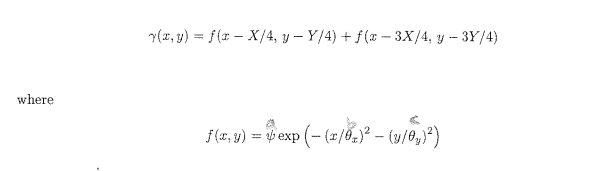
\includegraphics[width=80mm]{MaxFoodFunction.PNG} \newline
which creates the following grid: \newline
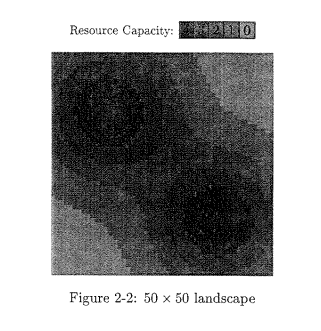
\includegraphics[width=80mm]{ResourceCapacity.PNG} \newline
%Validation
\newline
The last object that we created was the event object. This object holds the type of an event, the time that the event takes place in the next-event simulation, and the id of the agent that it relates to. If the type of the event is birth, it also holds the id numbers of the agents that are havung the child.
\newline
%Validation
\newline

\center 
Experiments and Data
\flushleft

Now that we had written our objects, we were able to create our simulation. We created a simulation method that took in the starting number of agents and the end time of the simulation. The first step of this simulation was to create an event of type ''check'' for every 5 units of time. An event of type ''check'' records the number of agents that are currently alive in the simulation and puts it into a list to be returned later. \newline
After this, we created a list of agents. When creating the agents, we created events for their beginning and end of fertility, as well as their death from old age. These events affect their agents by making them fertile, ending their fertility, and killing them.
\newline
It also creates their first movement event. To do this, we took the agent's feild of view (refer to this as FOV) to find the location with the most food that is within this range. We looked at All of the spots that were FOV steps to the left, right, in front of, and behind the the agent and found the location with the most food. The amount of time that it takes to move to the location is 0.5 + Exponential(0.5) per space. When the agent gets to its desired location, it picks up all of the food and searches to see if a mate is in range. It searches the same way that it searches for food, by looking left, right, forward, and backwards within the range of FOV. If the agent is fertile, and it finds an agent of the opposite gender who is fertile, whose pregnancy variable is false, and who can spare food for a child, then the two agents cannot move for 0.75 time intervals. They're pregnancy variables become true, and each agent needs to give 50 units of food (half of the starting value). An event of type birth is created for 0.75 time intervals after the current time, which creates another agent and the events that go with creating an agent. Then the parent agents' pregnancy variables become false again, and they continue living. \newline
The events are sorted by time and are carried out in that order. When new events are added, the events list is re-sorted to keep them in order.
\newline
The first time we ran the simulation, we did not use evolution. This means that agents did not pass traits on to their children. Running this simulation in this form with 500 starting agents resulted in the following graph, which represents the average population of the simulation for each 5 units of time for 10,000 simulations (The results are not continuous. The line is only there to make visualizing the pattern easier)\newline
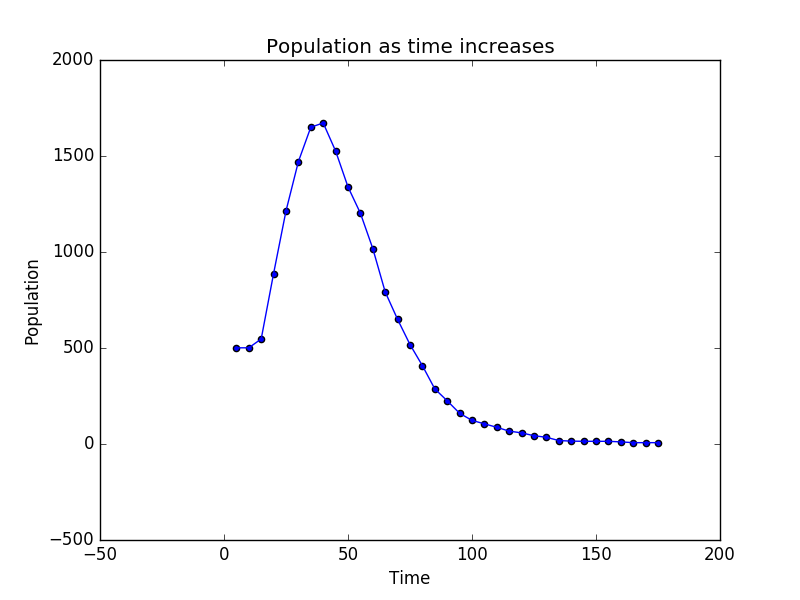
\includegraphics[width=80mm]{Population500noevo.png} \newline
This result appears to show that our agents are not able to keep the population alive. The population appears to peak at around the 45$^{th}$ or 50$^{th}$ time interval, which is around the median age of fertility for the first generation of agents. This pattern did not change significantly when we changed the amount of agents that the simulation started with. We also wanted to see how the simulation would run with evolution. In other words, the parents pass their traits on to their children. Here are the results: \newline
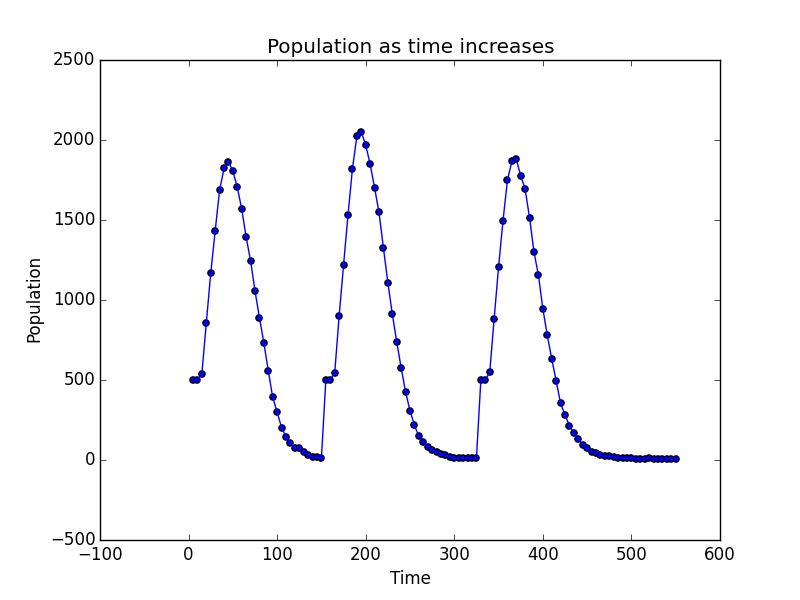
\includegraphics[width=80mm]{Population500.png} \newline
The population died out sooner, but went up to a higher level. \newline
Reproduction seems to stop at the same point as it did without evolution.
This lead us to believe that the first generation of agents were reproducing much more than the later generations. Either the newer generations could not find as many fertile agents, or the food was not replenishing quickly enough. We decided to find out which factor was making it difficult for the agents to reproduce.
\newline
To do this, we kept a counter of the reasons that agents of opposite genders were meeting without reproduction. These reasons included seeing an agent that was already pregnant, not having enough food to support a child, and not being fertile. We also kept track of how many times we checked if a pregnancy was possible. When we did this, we also recorded these levels each time that we checked the population, so that we could see how the increase of these levels accelerates as the simulation progresses. These are the results: \newline
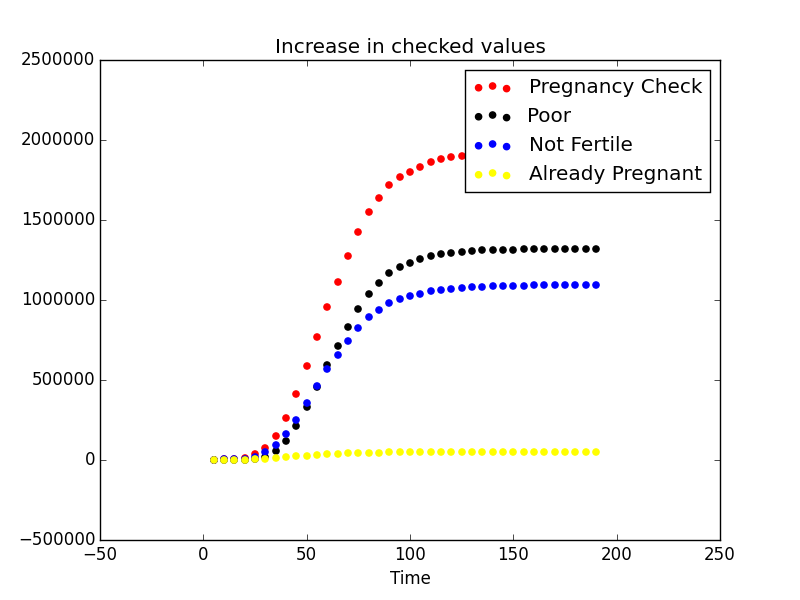
\includegraphics[width=80mm]{factors500.png} \newline
This graph shows that the amount of times that the agents were too poor accelerated more quickly than the amount of times agents were not fertile, so the low amount of resources seems to be doing more damage than fertility, so we doubled the food capacity in each location and made it replenish twice as fast. Here are the results: \newline
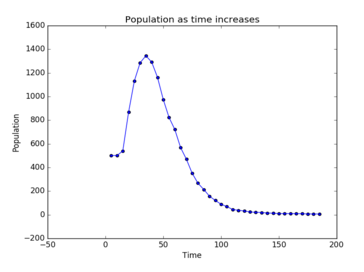
\includegraphics[width=80mm]{FoodCange.PNG} \newline
Increasing the food did not save the population, and even killed them off sooner, so we changed it to its original form and increased the length of fertility. To increase the length of fertility, the men ended fertility at Uniform(50, 60) and women ended at Uniform(60, 70). These are the results: \newline
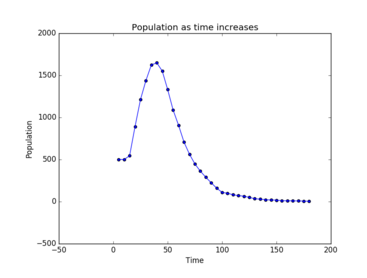
\includegraphics[width=80mm]{FertChange.PNG} \newline
The population lasted longer, but still died out. We then ran a simulation with increased food and fertility. Here are the results: \newline
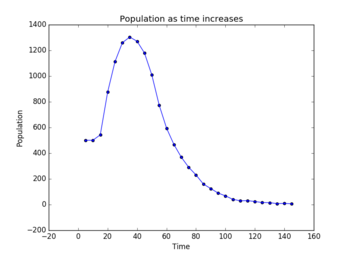
\includegraphics[width=80mm]{both.PNG} \newline
The population still dies out. \newline
\center 
Results and conclusions
\flushleft
From our experiments, we saw that evolution did help the population last longer, but the population seems to die off due to lack of food and fertility. We were not able to find a solution to save the population, but we would like to continue our research to find out what else we can change.









\end{multicols}

\end{document}